\section{Methods}

To see whether sexual reproduction is indeed preferred over asexual reproduction in a fast changing environment, an Artificial Life simulation was designed in Java. In this simulation, NEAT was used as an algorithm to evolve recurrent neural networks, which will be the brains of the agents.

\subsection{Simulation}

The simulated world is a simple 2D world with both food and poison represented by different colors.
In the environment, the agents will move around and eat food to collect energy.
The simulation is completely written in Java\footnote{For source code, see \url{http://github.com/g0ulash/NEATSimulation } NOTE: THIS GitHuB IS STILL PRIVATE}.

\subsubsection{Environment}

The environment consists of an empty field where food and poison are randomly spawned away from other food and agents - see Figure \ref{fig:env} for an example.
The environmental changes will be the food and poison, which will have some chance of switching and changing in value resulting in food becoming poison and vice versa. 
Obviously, nutrient food gives agents energy and poisonous food reduces the energy of an agent.
The amount of food will always be kept constant, so if one piece disappears there will be a new spawned piece of food on a random place.
There are also the borders, which enclose the environment.
If an agent collides with the border it will also lose energy.

\begin{figure}[H]
\centering
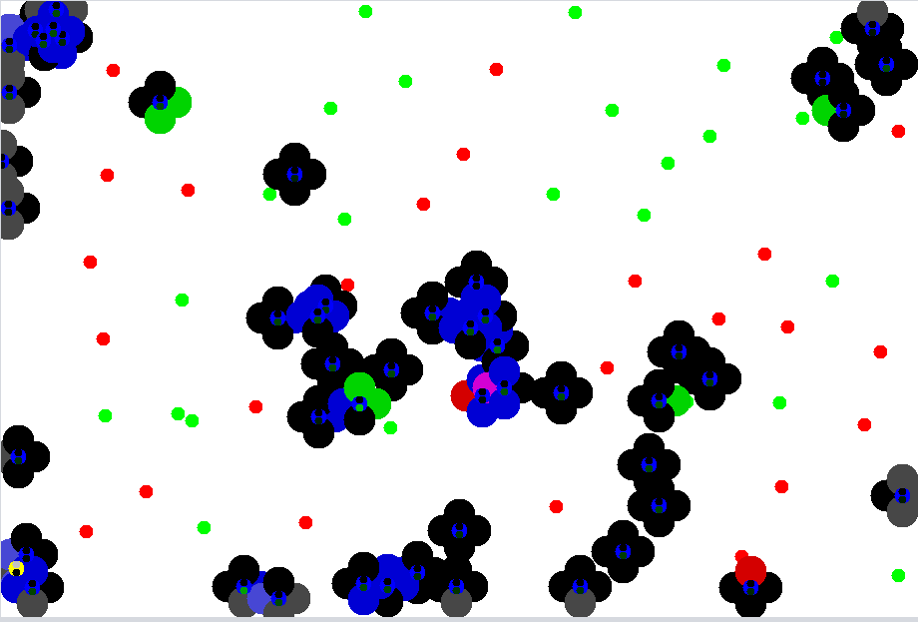
\includegraphics[scale=0.5]{environment.png}
\caption{An environment filled with agents, poisonous and nutricious food.}
\label{fig:env}
\end{figure}

\subsubsection{Agents}

Each agent, see Figure \ref{fig:agent} for an example, will have a recurrent neural network as a brain, which will be evolved using the NEAT algorithm.
They will inhabit this environment and have an extra evolvable parameter that determines whether they will reproduce sexually or asexually. 
The age of the agents is the number of iterations that it has been alive, which will also be the fitness function.
Each iteration, agents lose energy and when their energy is fully depleted, they will die.
So their goal is to try and find nutrient food and avoid poison to replenish their energy.
Agents can then reproduce if they surpass a certain energy threshold.
If they reproduce asexually they can only create offspring with mutation, while if they reproduce sexually they can create offspring with cross-over and mutation. 

The input to the neural network of each agent are four color sensors for each direction that can read the pixel value next to them.
Each color sensor is an RGB valued sensor, which results in $12$ input represented as floats.
The last input will be their own energy level, which makes it a total of $13$ inputs.
The output will be their movement which are output as 2 dimensional coordinates.
The activation function of the neural network is a hyperbolic tangent. 

\begin{figure}[H]
\begin{subfigure}[b]{0.5\linewidth}
    \centering
    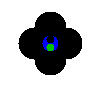
\includegraphics{agent_nofood.png}
\end{subfigure}%
\begin{subfigure}[b]{0.5\linewidth}
    \centering
    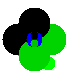
\includegraphics{agent_food.png}
\end{subfigure}
\caption{Agents as represented in the simulation. The left agent is an agent in rest state, which has nothing surrounding to sense and the right agent is one that senses food.}
\label{fig:agent}
\end{figure}

\subsubsection{Updates}

The number of the agents in the environment is kept constant.
For example, if two agents die then two new offsprings are created using NEAT.
The agents that will be selected using roulette wheel selection, where the probability of selecting an agent is proportional to his fitness function, which is the age of an agent.

\subsection{NEAT}

To implement the NEAT algorithm, we will refer to the original paper \cite{stanleyneat}.
Modeling and evolving Artificial Neural Networks (ANNs) in a genetic algorithm is not trivial, because the structure of different neural networks are not necessarily related.
To perform crossover operations, the network structures have to be analyzed to find appropriate crossover points, and naturally the genomic representations for ANNs do not clearly show where these points are.
With NEAT the authors have tried to overcome this problem by encoding history in each element of every single genome.
This guarantees that structures are identifiable and thus analyzed more easily.

Each genome in the algorithm consists of a list of nodes and a list of arcs.
Each arc has values for its input node, output node, the weight on the arc, whether the link is enabled or not and a so called innovation number.
The innovation number is the historical value, which allows the crossover operations to detect if the gene is similar to another gene in a different genome.
Each node contains a unique identification number, activation response threshold, whether it is enabled or not and also an innovation number.

\begin{figure}[H]
\centering
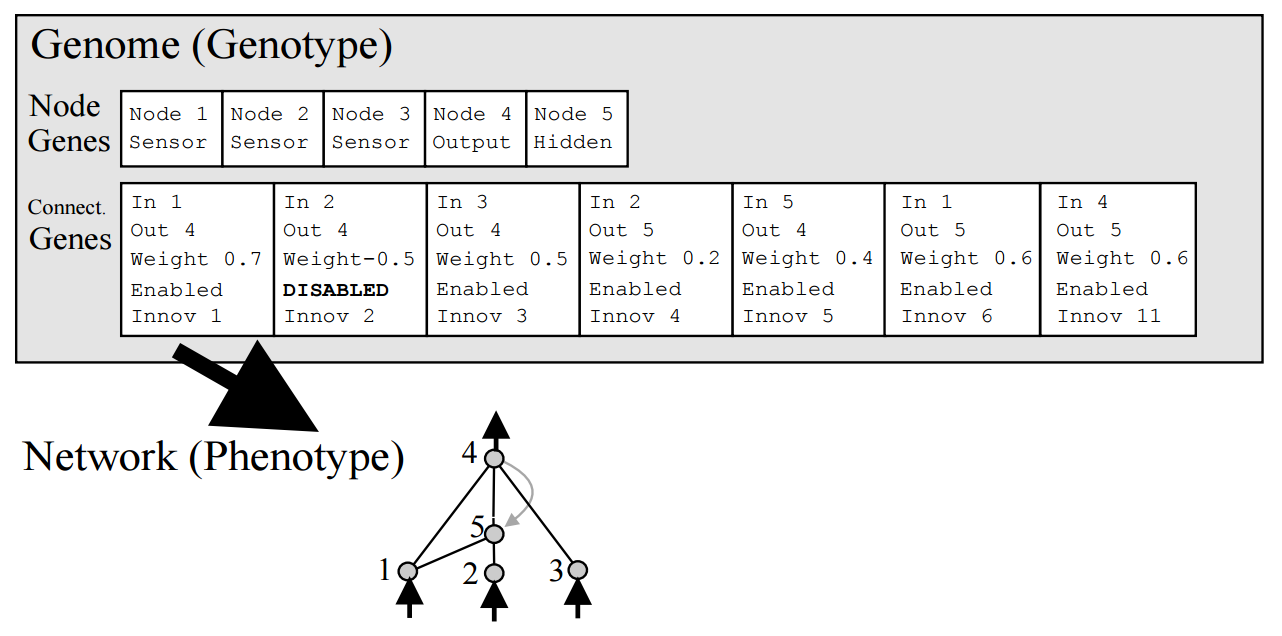
\includegraphics[width=\textwidth]{genopheno.png}
\caption{Genotype to phenotype mapping in NEAT.}
\label{fig:gen}
\end{figure}

Mutation can occur randomly in NEAT and it can change arc weights, activation thresholds and the network topology.
The weights and thresholds can be changed when a random arc or node is chosen and the values are constrained.
The network topology changes by randomly adding nodes or arcs.
When an arc mutation occurs, the algorithm first randomly selects two nodes.
If there did not exist an arc yet, it will then insert an arc with initial weight one.
If an arc already existed, the only thing it will do is enable the arc again if it was disabled.
And a last special case, if there is no arc between the two nodes, but an equivalent arc is already present in another genome of the population, this arc will be copied with the same innovation number - the reason for this is that it is not a new innovation.
Mutation of nodes arrives in another fashion, as instead of randomly choosing two nodes, the algorithm now takes an arc, disables it and also adds a new node.
This node, with a random activation threshold, will be connected to the nodes that were connected to the disabled arc - effectively creating two new arcs as well.
The weight of the disabled arc will be copied to the output arc of the new node and the weight of the input arc will be set to one, such that it does not interfere with any learning that has taken place, yet.

\begin{figure}[H]
\centering
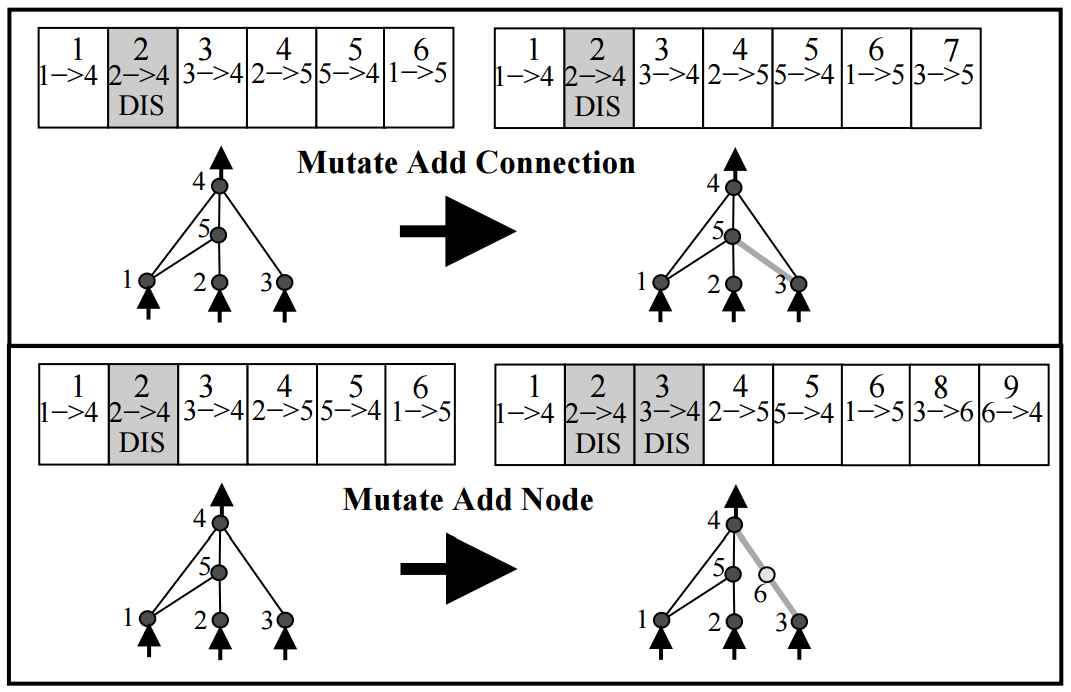
\includegraphics[width=\textwidth]{mutation.png}
\caption{The two types of mutation in NEAT.}
\label{fig:mut}
\end{figure}

Before crossover can be introduced, the innovation numbers have to be explained.
Since the innovation numbers are not unique to genes specifically but only to the innovation (i.e. new gene), you can compare two genomes in the population and check if they share any genes.
If any of the genes share the same number, they also share the same manifestation. 
NEAT stores the innovations in a database that have occurred since the initial population.
Before a new innovation is introduced, the database will be checked if it does not already exist.
If it is a new innovation, the database will store the innovation and increment a global innovation number which will pass on to that gene.
This ensures that all related genes are eventually identical.

When a crossover operation is applied to two genomes, the new genome will receive the same innovation numbers in the genes.
Because NEAT uses these innovation numbers, it can easily align two genomes to see which parts are similar and which are different.
The genes that have different innovation numbers are called disjoint and added to the child during crossover.
Genes that have newer innovation numbers are called excess and also added to the child during crossover.
The genes that have shared innovation numbers are inherited by the parent genome that has the highest fitness value.
The crossover operations in this algorithm limit the support for big diversity, as a new innovation, which can have a high impact, can be erased from the population before it reaches its potential.

To overcome this problem, NEAT uses speciation.
In nature, speciation is defined as when two organisms once shared a genome sometimes diverge such that they can no longer mate with each other.
When a genome diverges far enough (according to a certain formula) from that of the other genomes in the population, NEAT will find this genome and put it in its own species.
It calculates the distance based on the excess and disjoint genes and the average weight differences of two genomes - each of these parameters are weighted.
The initial population consists of one species.
Following new generations, NEAT can identify a genome that should be in a new species and makes one accordingly.
If other genomes in one species are diverging from their own species towards another, the algorithm will transfer this genome between species.
Through certain fitness testing, NEAT can identify whether or not new genomes in a species have improved fitness compared to the original genome in that species.
If a species has not improved over a certain amount of generations, it can be deleted entirely from the population - because this means that a certain innovation did not have enough impact.
Based on the fitness value of the species, each species will have a percentage of spots for the new generation.

\begin{figure}[H]
\centering
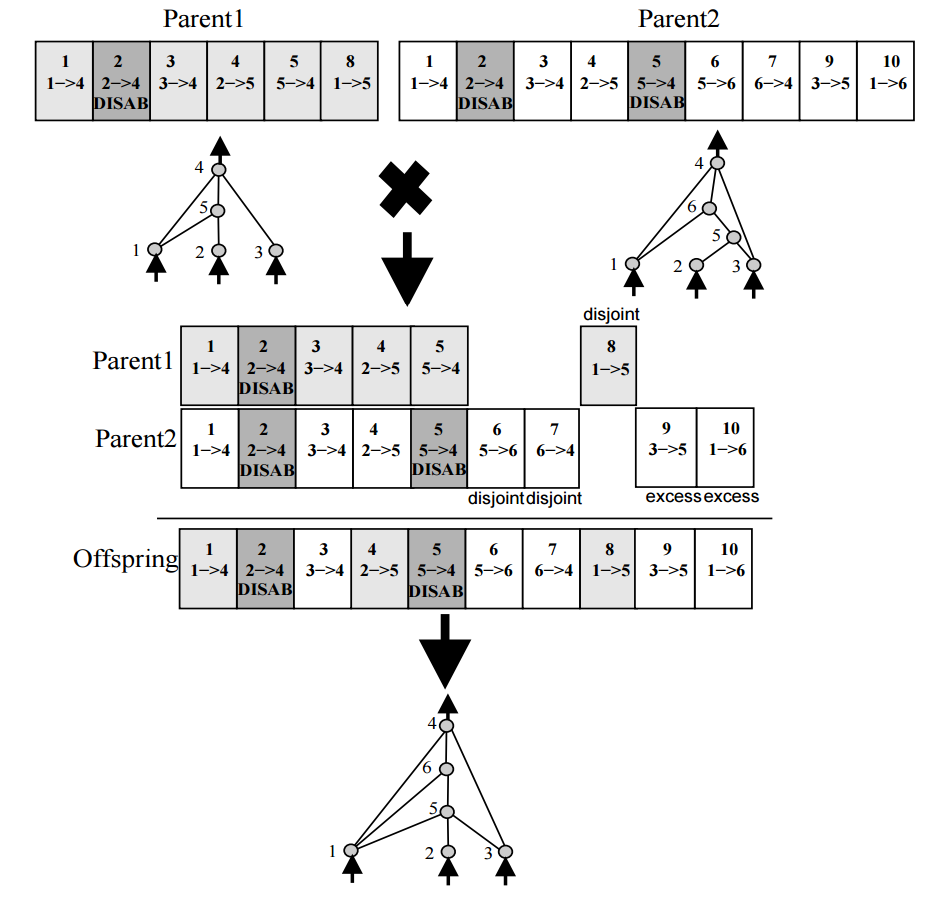
\includegraphics[width=\textwidth]{crossover.png}
\caption{Crossover as it is specified in NEAT.}
\label{fig:cross}
\end{figure}

\subsection{Analysis}
There will be two experiments, one where the environment changes slowly and one where it will change more rapidly. 
Thus in a rapid changing environment poison and food will switch more frequently and with higher magnitude than in a slow changing environment.
Ideally there will be multiple experiments, where the pace of changes in the environment is increased in small steps.
In this way the results could show if there is a certain turnover point where the sexual reproduction starts becoming advantagouos, if our hypothesis is correct.
However, this will only be possible to be tested if there is enough time.